\documentclass[a4paper,11pt]{report}
%\usepackage{hyperref}
\usepackage{setspace}
\usepackage{url,natbib,amssymb,hyperref,graphicx,wrapfig,setspace,multirow,booktabs,subfig,array,wrapfig,calc}
\usepackage{array}
\newcolumntype{P}[1]{>{\centering\arraybackslash}p{#1}}
\usepackage{fancyhdr}
\usepackage{color}
\usepackage{booktabs,caption,fixltx2e}
%\usepackage[round]{natbib}      % References with names and years
%[round]
\usepackage{xr}                 % reference anothe chapter
%\externaldocument[2-]{../CHAPTER2/ch2_LSM_v11}
%\externaldocument[3-]{../CHAPTER3/ch3_sensitivity_v10}
\usepackage{graphicx}
\usepackage{caption}
\usepackage{appendix}
%\usepackage{subfigure}
\usepackage{float}
\usepackage{subfig}
\usepackage{float}
\usepackage{paralist}                % inline lists
\usepackage{gensymb}    % degrees celsius as {\celsius}
%\usepackage{textcomp]    % arrows
\newcommand{\tildetext}{\raise.17ex\hbox{$\scriptstyle\mattt{\sim}$}}
\usepackage{rotating}   %rotate table
%\renewcommand{\arraystretch}{1.5}  %increase space between rows in tables (default is 1) because there is already baselinestrech 1.5 tables become too separated, maybe with normal spacing this command should be used
\usepackage{rotating,booktabs}
\usepackage{threeparttable}
\usepackage{multirow}
\usepackage{color}% color the text
\usepackage{amsmath}
\usepackage{textcomp}
% Page setup from thesis template
\topmargin=-10mm
\textwidth=150mm
\textheight=234mm
\headsep=12mm
\oddsidemargin=14mm
%\oddsidemargin=12mm
\evensidemargin=-1mm
%\evensidemargin=1mm
\parindent=6mm
\parskip=1em 

\newlength{\rulewidth}
\setlength{\rulewidth}{150mm} % change to 150mm for printing on
			      % gordon, 149 otherwise???
% 1.5 line spacing so my supervisor can scrawl all over it
\renewcommand{\baselinestretch}{1.50}

\pagestyle{headings}    % chapter number on top

\setcounter{secnumdepth}{4}              %Numbers subsubsections, and lower.
\setcounter{tocdepth}{4}                 %Sets depth of table of contents to include subsubsections.

\pagestyle{fancy}
\fancyhf{}
%\rhead{\fancyplain{}{\textit{\nouppercase\rightmark}}}
\fancyhead[L]{Chapter 5. Deriving vegetation architectural parameters from observed data}
\fancyfoot[C]{ \thepage\ }

%opening
\title{}
\author{Renato Kerches Braghiere \\ This document was written in \LaTeX \\ Number of words: 12213}
\date{\today}

\begin{document}
\maketitle
\setcounter{chapter}{4} %so next one is 4

\chapter{Deriving vegetation architectural parameters from observed data}

\section{Introduction}\label{introduction}

The main purpose of this chapter is to explore observational methods to access vegetation structural variables, and how to derive the structure factor parameters from observed data.  To do so, this chapter intends to address three main points: i) to explore different methods of measuring the radiative partitioning over predetermined sites (Tonzi Ranch and one BOREAS site – Southern study site), and compare them; ii) to derive the structure factor parameters from digital hemispherical photographs and evaluate their theoretical impacts on radiation partitioning for all evaluated sites (Tonzi Ranch, 3 BOREAS sites, 2 Oregon sites, and Alice Holt); iii) To compare modelled radiation partitioning with and without the structure factor parameterisation and, when available, compare with observed data.

\section{Addressing gap fraction}\label{section:hemiphotos}

This section explores different methods of measuring/simulating radiation partitioning, i.e., absorptance, reflectance, and transmittance through the characterisation of direct transmissivity, or the gap fraction. The gap probability theory is used in this section as a method to derive the relevant variables of the clumping index of Nilson, and the structure factor of Pinty. As a first step, this section makes a comparison study between different ways of observing direct transmissivity. This is important because it shows something about i) area of applicability of a determined method, and ii) the reason why the methods agree, or disagree.

Experiment 1. For Tonzi Ranch, BOREAS-SSA, and BOREAS-NSA, the gap probability were acquired in two different ways:
\begin{enumerate}
\item Digital Hemispherical Photographs;
\item 3D model with structural data derived from Airborne LiDAR.
\end{enumerate}
The gap fraction was extracted from both of them in two different ways described in methodology, but summarised here. For 1), the pictures were thresholded and averaged. For 2), a 3D model was used and the canopy was set to be black.

\subsection{Tonzi Ranch}

Tonzi Ranch (latitude: 38.4318N; longitude: 120.9668W; altitude: 177 m) is located in the lower foothills of the Sierra Nevada Mountains, Ione, CA, USA, and it is part of
the AmeriFlux (http://public.ornl.gov/ameriflux/). It is classified as an oak-grass savanna woodland on flat terrain (average slope: 1.58$^{\circ}$), and experiences Mediterranean-type climate with dry, hot summers and rainy, mild winters. Annual average temperature and annual precipitation are 16.9 $^{\circ}$C and 565 mm, respectively (1949 - 2005 climate normals from Camp Pardee climate station; latitude; 38.258N; longitude: 120.858W). The overstory consists of dominant blue oak trees (\textit{Quercus douglasii}) with occasional ($<$10\%) grey pine trees (\textit{Pinus sabiniana}). The understory is mainly composed of grasses and forbs (\textit{Brachypodium distachyon}, \textit{Hypochaeris glabra}, \textit{Bromus madritensis}, \textit{Cynosurus echinatus}) \citep{Baldocchi2004}. Due to the low density of grey pine trees (\textit{Pinus sabiniana}), it is assumed no element clumping (related only to needle-to-shoot strcuture). The stem density was 144 ha$^{-1}$, tree height was 9.4 $\pm$ 4.3 m (mean $\pm$ stanstandard deviation), trunk height was 1.8 $\pm$ 1.3 m, diameter at breast height (DBH) was 0.26 $\pm$ 0.11 m, mean crown radius was 2.9 $\pm$ 1.4 m, and canopy cover was 0.47 \citep{Chen2008}. More detailed site information may be found in previous studies \citep{Baldocchi2004,Ma2007,Chen2008}. DHPs were acquired by \citet{Ryu2010} from 5$^{th}$ to 7$^{th}$ of August, 2008, close to the peak of the growing season, on a 300 m $x$ 300 m sampling plot with the flux tower at the centrer, gridded at 30 m $x$ 30 m intervals. The extent of the plot corresponds to the scale of spatial heterogeneity as determined through semivariogram analysis \citep{Kim2006}. 

Direct transmissivity was extracted from the DHPs using the CIMES-FISHEYE software \citep{Walter2012}. First, the raw photographs were oriented to the geographic North; East and West are inverted on Hemispherical Photographs (East left, West right). Second, the horizon circle of the image have to be identified, and to do so, brightness should be increased, and contrast adjusted. Third, the pixel coordinates of 3 points clearly defined on the inner border of the circle are enough to describe the hemisphere of the photograph. The coordinates are used in the software to centre the image and define its circular limit. For this set of DHPs, there was no need to repeat this procedure for other images, since their position and diameter did not vary from one image to the next. Fourth, colour digital images are made of pixels, and pixels are made of combinations of primary colours. A channel in this context is the grayscale image of the same size as a colour image, made of just one of the primary colours. For instance, an image from a standard digital perspective will have a red, a green, and a blue channel, or RGB. A grayscale image has just one channel. The green channel translates best halftones but is not suited for analysis. The red and blue channels offer good contrast separating sky (background) from plants (foreground). Usually for analysis, the blue channel is selected (Figure~\ref{f:bluepic}) and the remaining channels are discarded. 

Fifth, the selection of an appropriate method to calculate a threshold is of concern to hemispherical photography analysis. Some softwares offers several methods to determine automatically a global threshold value derived from the histogram of grey levels of the whole image \citep{Ridler1978}. In fact, there is no perfect thresholding method, therefore, to ensure consistency, it is important to always use the same method for a given set of photographs. It allows repeatability of the process, independent of any user. For Tonzi Ranch the chosen threshold was globally set to 195. However, under bright light conditions, the threshold was increased, and under dark light conditions the threshold was decreased. Within 52 photographs, 12 presented abnormal light condition (either too bright, or too dark). The other 40 photographs were set at 195 threshold. The final step is converting the grey-toned image to a binary (classified) image, where black pixels represent foliage and white pixels sky.

\begin{figure}
\centering

\begin{tabular}{ll}
\subfloat[Original DHP]{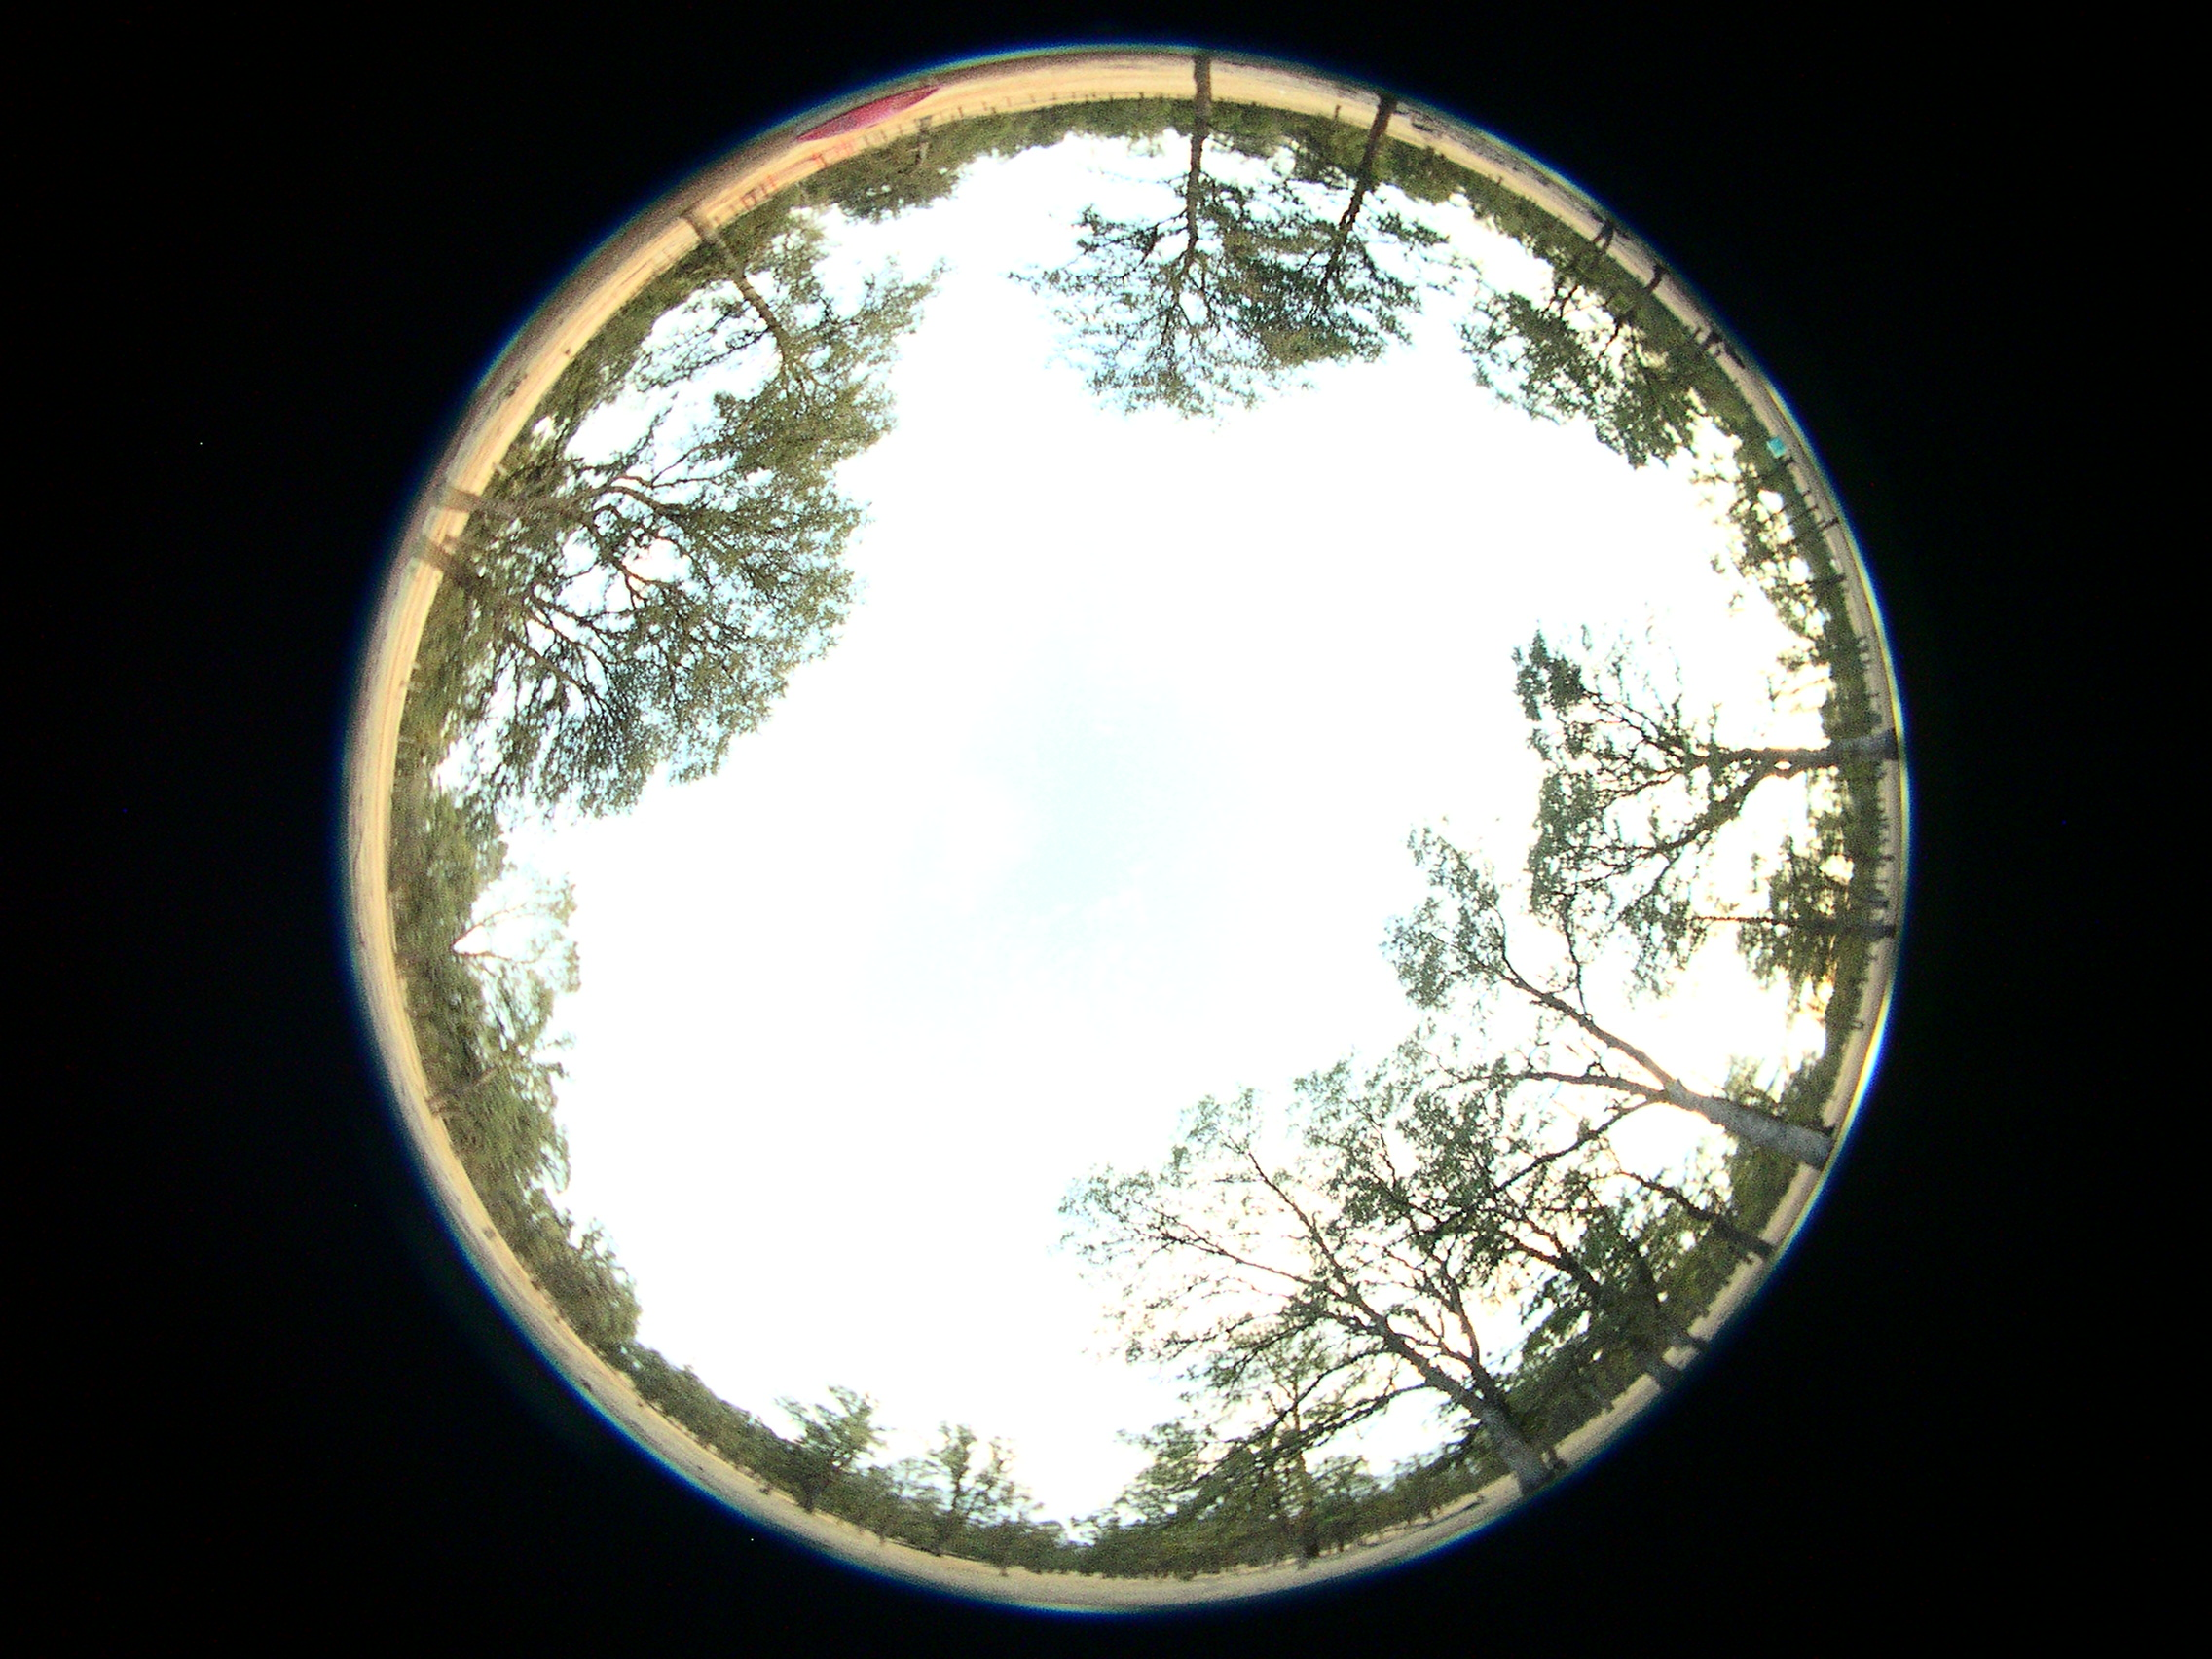
\includegraphics[width=0.5\textwidth]{/home/mn811042/Thesis/chapter5/figures/original.jpg}}
\subfloat[Thresholded DHP]{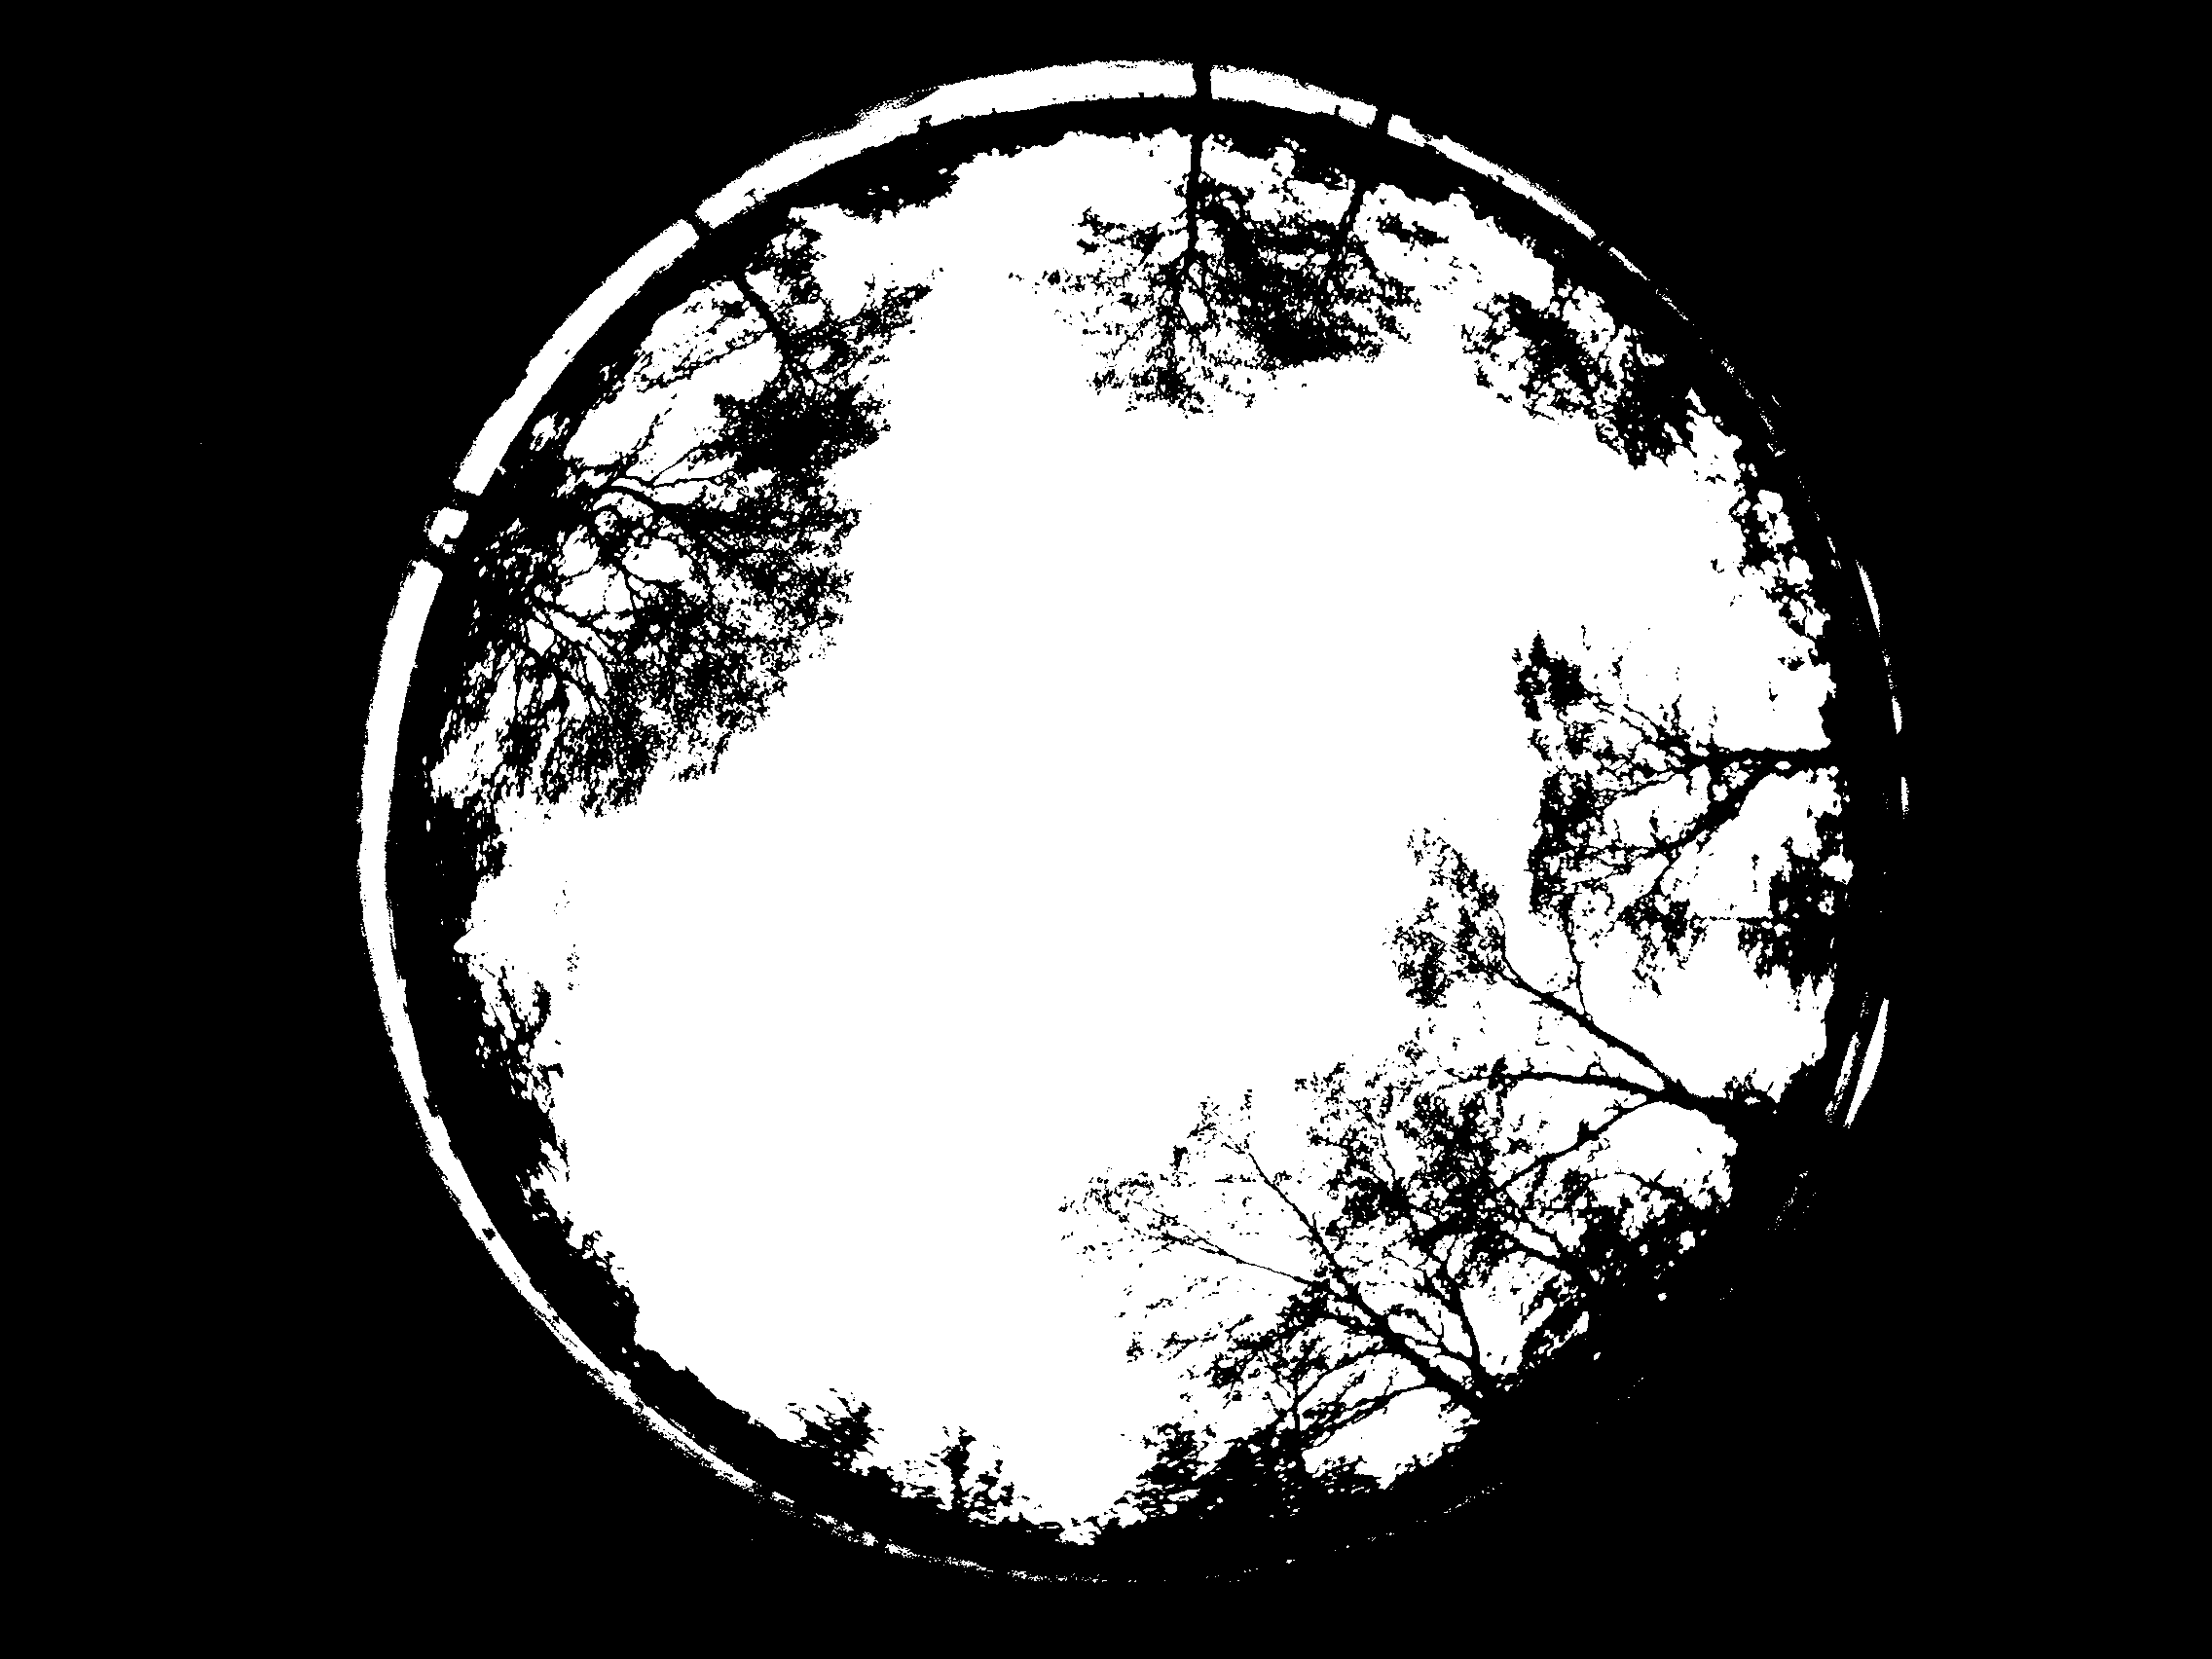
\includegraphics[width=0.5\textwidth]{/home/mn811042/Thesis/chapter5/figures/dhp01.png}}
\end{tabular}

\begin{tabular}{ll}
\subfloat[P$_{gap}$($\phi$,$\theta$)]{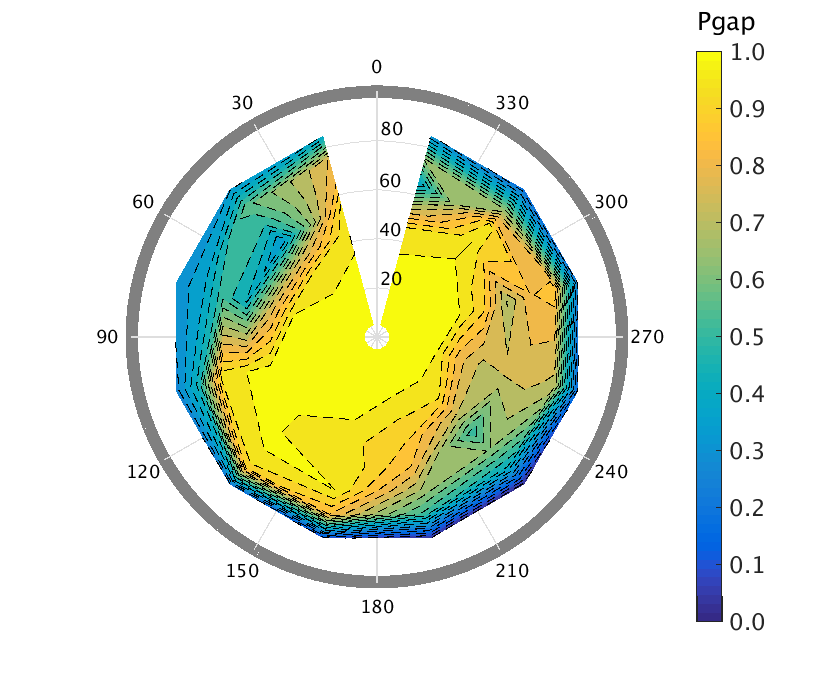
\includegraphics[width=0.5\textwidth]{/home/mn811042/Thesis/chapter5/figures/DHP01_9_12_2.png}}
\subfloat[P$_{gap}$($\theta$)]{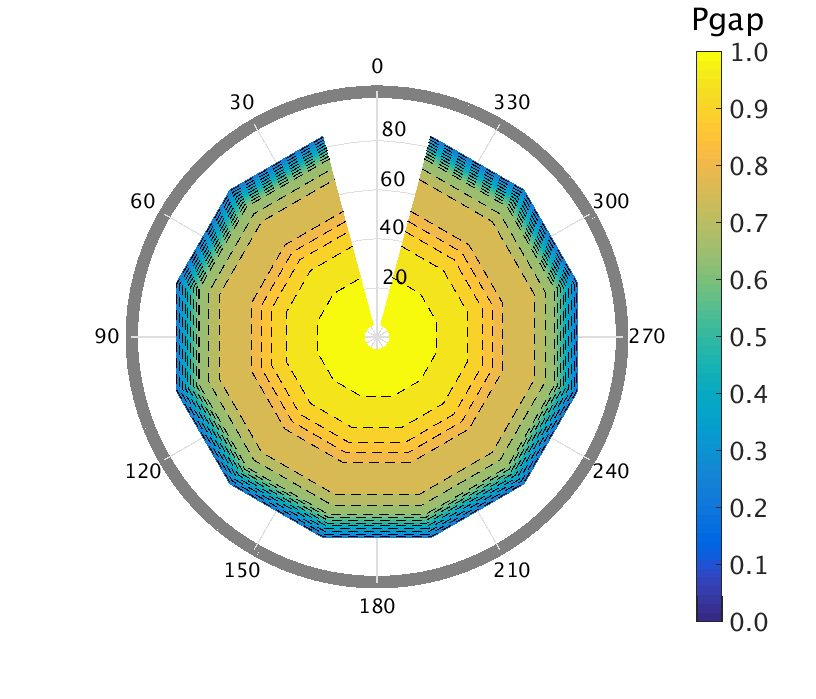
\includegraphics[width=0.5\textwidth]{/home/mn811042/Thesis/chapter5/figures/DHP01_9_12_average.png}}
\end{tabular}

\caption{a. Hemispherical photograph taken on the 6$^{th}$ (sunset) of August, 2008, at the Tonzi Ranch \citep{Ryu2010}; b. Digital Hemispherical Photograph in the blue channel after threshold = 195 and classified into a binary 8-bits image (black and white); c. gap fraction (P$_{gap}$($\phi$,$\theta$)), with 108 segments (9 zenith angles x 12 azimuth angles). Note the inversion of E and W; d. gap fraction (P${_gap}$($\theta$)) averaged over the azimuth ($\phi$) for each zenith angle. } 
\label{f:bluepic}
\end{figure}

Thus, gap fraction over a given area is computed from a digital image classified into black (B) and white (W) pixels separating sky and canopy elements. If, for example, $B$ represents canopy elements and $W$ sky on a positive image, gap fraction is calculated as:

\begin{equation}
P_{gap}(\phi,\theta) = \frac{P_W}{(P_W + P_B)}}
\label{equation:rmseab}
\end{equation}

\noindent where $\phi$ is the mid-point of azimuth angle of a portion of the hemisphere projected to the image plane, $\theta$ is the mid-point of zenith angle, P$_B$ is the number of black pixels, and P$_W$ the number of white pixels contained in that sector. Therefore, in hemispherical photography, gap fraction represents the relative proportion of open sky contained in any defined region on the projected image plane \citep{Frazer1997}.

The projected image plane is divided into elements of a sampling grid, according to the geometric distortion of the fisheye lens, and the image plane is divided into equiangular annuli from zenith to horizon and equiangular azimuth sectors, which determine sky divisions, or segments.

The P$_{gap}$ for all DHPs plus the mean and the 95\% confidence intervals are represented in Figure~\ref{f:pgaptonzi}.

\begin{figure}
\centering
\begin{tabular}{lll}
%\subfloat[Original DHP]{\includegraphics[width=0.33\textwidth]{/home/mn811042/Thesis/chapter5/figures/Pgap_average_tonzi.png}}
\subfloat[5x18]{\includegraphics[width=0.33\textwidth]{/home/mn811042/Thesis/chapter5/figures/Pgap_average_tonzi_18.png}}
\subfloat[Original DHP]{\includegraphics[width=0.33\textwidth]{/home/mn811042/Thesis/chapter5/figures/tonzi_adj_nilson.png}}
\subfloat[5x18]{\includegraphics[width=0.33\textwidth]{/home/mn811042/Thesis/chapter5/figures/tonzi_adj_pinty.png}}
\end{tabular}


\caption{a. Hemispherical photograph taken on the 6$^{th}$ (sunset) of August, 2008, at the Tonzi Ranch \citep{Ryu2010}; b. Digital Hemispherical Photograph in the blue channel after threshold = 195 and classified into a binary 8-bits image (black and white); c. gap fraction (P$_{gap}$($\phi$,$\theta$)), with 108 segments (9 zenith angles x 12 azimuth angles). Note the inversion of E and W; d. gap fraction (P${_gap}$($\theta$)) averaged over the azimuth ($\phi$) for each zenith angle. } 
\label{f:bluepic}
\end{figure}

To invert the P$_{gap}$ the correct estimation of LAI is really important and can affect the final results quite substantially. For Tonzi Ranch, many different sources of data were provided to determine an average ecosystem LAI. \citet{Ryu2010} determined a maximum tree LAI of 0.77 $\pm$ 0.27, while LiDAR data \citep{Chen2008} gave a result of 0.7 $\pm$ 0.4 for average individual tree LAI. Other estimates of LAI were made by Nancy Kiang, using the LI-2000 and by litterbags collected by John Battles group estimating a overestory LAI of 0.65 on the 1$^{st}$ of August. Finally, the IKONOS, Lidar altimeter assessed seasonal LAI trends for over and understory with values around 0.7 from the end of the growing season in May. For this study, a LAI of 0.7 was considered.



\subsection{BOREAS}
Hemispherical photographs were acquired in sample arrays at heights of 0.8, 1.5, and 2.5 m for each of the forested BOREAS tower flux sites and auxiliary sites. For the forested tower flux sites and other sites for which mapped plots were set up, hemispherical photographs were acquired during IFC-1 and IFC-2 at 10 m intervals along the central X axis of the mapped plot (5 m intervals for NSA-YJP). Typically, this corresponds to six sample locations for each tower flux site. Site locations in relation to the flux tower (Figure 1) are SOBS, 150-230 m (SE); SOJP, 130-180 m (SE); SYJP, 30-80 m (SE); SOA, 70-120 m (SW); NOBS, 80-130 m (SE); NOJP, 70-120 m (SE); and NYJP, 120-150 m (SE). Location refers to distance from the flux tower along the “B” LA1 transect, except in the case of SOBS, where a “D” line (20 m from the C line) is used. For the auxiliary sites, hemispherical photographs were taken in a crisscross array, at 10 m intervals along two 40 m long transects placed at right angles and crossing in
the middle. A total of nine sample locations were chosen within the plot. The auxiliary site photographs were taken during and between IFC-1 and IFC-2.
Hemispherical photograph negatives were video digitized at a resolution of 512 (horizontal) X 480 (vertical) X 7 bits using the hemispherical photograph analysis system CANOPY (Rich, 1989, 1991). Gap fraction, the proportion of unobstructed sky, was calculated at 5$^{\circ}$ zenith angle intervals and used for additional calculations. All hemisphericai photographs were also archived in Kodak PhotoCD format. The effective LA1 and other canopy indices were calculated using the program LAICALC. Calculating formulae and operation of LAICALC are described in detail in the LAICALC manual [Rich et al., 19951 following the method of Chen et al. [1991]. In order to compare hemispherical photography technique and LAI-2000 results, the gap fractions from the photographs were similarly separated into five zenith angles from 0 to 75$^{\circ}$.

\bigskip
\noindent\textbf{NSA-OBS-FLXTR}
\bigskip

PAI = 4.95 from TRAC; date: 10$^{th}$ June 1994

\begin{figure}
\centering
\begin{tabular}{lll}
%\subfloat[Original DHP]{\includegraphics[width=0.33\textwidth]{/home/mn811042/Thesis/chapter5/figures/Pgap_average_tonzi.png}}
\subfloat[5x18]{\includegraphics[width=0.33\textwidth]{/home/mn811042/Thesis/chapter5/figures/Pgap_average_NSA-OBS-FLXTR.png}}
\subfloat[Original DHP]{\includegraphics[width=0.33\textwidth]{/home/mn811042/Thesis/chapter5/figures/NSA-OBS-FLXTR_adj_nilson.png}}
\subfloat[5x18]{\includegraphics[width=0.33\textwidth]{/home/mn811042/Thesis/chapter5/figures/NSA-OBS-FLXTR_pinty.png}}
\end{tabular}
\caption{a. Hemispherical photograph taken on the 6$^{th}$ (sunset) of August, 2008, at the Tonzi Ranch \citep{Ryu2010}; b. Digital Hemispherical Photograph in the blue channel after threshold = 195 and classified into a binary 8-bits image (black and white); c. gap fraction (P$_{gap}$($\phi$,$\theta$)), with 108 segments (9 zenith angles x 12 azimuth angles). Note the inversion of E and W; d. gap fraction (P${_gap}$($\theta$)) averaged over the azimuth ($\phi$) for each zenith angle. } 
\label{f:bluepic}
\end{figure}


\bigskip
\noindent\textbf{NSA-OJP-FLXTR}
\bigskip

PAI = 2.25 from TRAC; date: 11$^{th}$ June 1994; DHPs collected on 13$^{th}$ July 1994

\begin{figure}
\centering
\begin{tabular}{lll}
%\subfloat[Original DHP]{\includegraphics[width=0.33\textwidth]{/home/mn811042/Thesis/chapter5/figures/Pgap_average_tonzi.png}}
\subfloat[5x18]{\includegraphics[width=0.33\textwidth]{/home/mn811042/Thesis/chapter5/figures/Pgap_average_NSA-OJP-FLXTR.png}}
\subfloat[Original DHP]{\includegraphics[width=0.33\textwidth]{/home/mn811042/Thesis/chapter5/figures/NSA-OJP-FLXTR_adj_nilson.png}}
\subfloat[5x18]{\includegraphics[width=0.33\textwidth]{/home/mn811042/Thesis/chapter5/figures/NSA-OJP-FLXTR_pinty.png}}
\end{tabular}
\caption{a. Hemispherical photograph taken on the 6$^{th}$ (sunset) of August, 2008, at the Tonzi Ranch \citep{Ryu2010}; b. Digital Hemispherical Photograph in the blue channel after threshold = 195 and classified into a binary 8-bits image (black and white); c. gap fraction (P$_{gap}$($\phi$,$\theta$)), with 108 segments (9 zenith angles x 12 azimuth angles). Note the inversion of E and W; d. gap fraction (P${_gap}$($\theta$)) averaged over the azimuth ($\phi$) for each zenith angle. } 
\label{f:bluepic}
\end{figure}



\bigskip
\noindent\textbf{NSA-YJP-FLXTR}
\bigskip

PAI = 1.61 from TRAC; date: 13$^{th}$ June 1994; DHPs collected on 17$^{th}$ July 1994

\begin{figure}
\centering
\begin{tabular}{lll}
%\subfloat[Original DHP]{\includegraphics[width=0.33\textwidth]{/home/mn811042/Thesis/chapter5/figures/Pgap_average_tonzi.png}}
\subfloat[5x18]{\includegraphics[width=0.33\textwidth]{/home/mn811042/Thesis/chapter5/figures/Pgap_average_NSA-YJP-FLXTR.png}}
\subfloat[Original DHP]{\includegraphics[width=0.33\textwidth]{/home/mn811042/Thesis/chapter5/figures/NSA-YJP-FLXTR_adj_nilson.png}}
\subfloat[5x18]{\includegraphics[width=0.33\textwidth]{/home/mn811042/Thesis/chapter5/figures/NSA-YJP-FLXTR_pinty.png}}
\end{tabular}
\caption{a. Hemispherical photograph taken on the 6$^{th}$ (sunset) of August, 2008, at the Tonzi Ranch \citep{Ryu2010}; b. Digital Hemispherical Photograph in the blue channel after threshold = 195 and classified into a binary 8-bits image (black and white); c. gap fraction (P$_{gap}$($\phi$,$\theta$)), with 108 segments (9 zenith angles x 12 azimuth angles). Note the inversion of E and W; d. gap fraction (P${_gap}$($\theta$)) averaged over the azimuth ($\phi$) for each zenith angle. } 
\label{f:bluepic}
\end{figure}

\bigskip
\noindent\textbf{SSA-9OA-FLXTR}
\bigskip

PAI = 4.63 from DHP (0.3 m); date: 02$^{nd}$ June 1994

\begin{figure}
\centering
\begin{tabular}{lll}
%\subfloat[Original DHP]{\includegraphics[width=0.33\textwidth]{/home/mn811042/Thesis/chapter5/figures/Pgap_average_tonzi.png}}
\subfloat[5x18]{\includegraphics[width=0.33\textwidth]{/home/mn811042/Thesis/chapter5/figures/Pgap_average_SSA-9OA-FLXTR.png}}
\subfloat[Original DHP]{\includegraphics[width=0.33\textwidth]{/home/mn811042/Thesis/chapter5/figures/SSA-9OA-FLXTR_adj_nilson.png}}
\subfloat[5x18]{\includegraphics[width=0.33\textwidth]{/home/mn811042/Thesis/chapter5/figures/SSA-9OA-FLXTR_pinty.png}}
\end{tabular}
\caption{a. Hemispherical photograph taken on the 6$^{th}$ (sunset) of August, 2008, at the Tonzi Ranch \citep{Ryu2010}; b. Digital Hemispherical Photograph in the blue channel after threshold = 195 and classified into a binary 8-bits image (black and white); c. gap fraction (P$_{gap}$($\phi$,$\theta$)), with 108 segments (9 zenith angles x 12 azimuth angles). Note the inversion of E and W; d. gap fraction (P${_gap}$($\theta$)) averaged over the azimuth ($\phi$) for each zenith angle. } 
\label{f:bluepic}
\end{figure}
\bigskip
\noindent\textbf{SSA-OBS-FLXTR}
\bigskip

PAI = 4.76 from TRAC; date: 29$^{th}$ July 1994; DHPs collected on 30$^{th}$ July 1994

\begin{figure}
\centering
\begin{tabular}{lll}
%\subfloat[Original DHP]{\includegraphics[width=0.33\textwidth]{/home/mn811042/Thesis/chapter5/figures/Pgap_average_tonzi.png}}
\subfloat[5x18]{\includegraphics[width=0.33\textwidth]{/home/mn811042/Thesis/chapter5/figures/Pgap_average_SSA-OBS-FLXTR.png}}
\subfloat[Original DHP]{\includegraphics[width=0.33\textwidth]{/home/mn811042/Thesis/chapter5/figures/SSA-OBS-FLXTR_adj_nilson.png}}
\subfloat[5x18]{\includegraphics[width=0.33\textwidth]{/home/mn811042/Thesis/chapter5/figures/SSA-OBS-FLXTR_pinty.png}}
\end{tabular}
\caption{a. Hemispherical photograph taken on the 6$^{th}$ (sunset) of August, 2008, at the Tonzi Ranch \citep{Ryu2010}; b. Digital Hemispherical Photograph in the blue channel after threshold = 195 and classified into a binary 8-bits image (black and white); c. gap fraction (P$_{gap}$($\phi$,$\theta$)), with 108 segments (9 zenith angles x 12 azimuth angles). Note the inversion of E and W; d. gap fraction (P${_gap}$($\theta$)) averaged over the azimuth ($\phi$) for each zenith angle. } 
\label{f:bluepic}
\end{figure}
\bigskip
\noindent\textbf{SSA-OJP-FLXTR}
\bigskip

PAI = 3.20 from TRAC; date: 30$^{th}$ May 1993; DHPs collected on 29$^{th}$ July 1994

\begin{figure}
\centering
\begin{tabular}{lll}
%\subfloat[Original DHP]{\includegraphics[width=0.33\textwidth]{/home/mn811042/Thesis/chapter5/figures/Pgap_average_tonzi.png}}
\subfloat[5x18]{\includegraphics[width=0.33\textwidth]{/home/mn811042/Thesis/chapter5/figures/Pgap_average_SSA-OJP-FLXTR.png}}
\subfloat[Original DHP]{\includegraphics[width=0.33\textwidth]{/home/mn811042/Thesis/chapter5/figures/SSA-OJP-FLXTR_adj_nilson.png}}
\subfloat[5x18]{\includegraphics[width=0.33\textwidth]{/home/mn811042/Thesis/chapter5/figures/SSA-OJP-FLXTR_pinty.png}}
\end{tabular}
\caption{a. Hemispherical photograph taken on the 6$^{th}$ (sunset) of August, 2008, at the Tonzi Ranch \citep{Ryu2010}; b. Digital Hemispherical Photograph in the blue channel after threshold = 195 and classified into a binary 8-bits image (black and white); c. gap fraction (P$_{gap}$($\phi$,$\theta$)), with 108 segments (9 zenith angles x 12 azimuth angles). Note the inversion of E and W; d. gap fraction (P${_gap}$($\theta$)) averaged over the azimuth ($\phi$) for each zenith angle. } 
\label{f:bluepic}
\end{figure}
\bigskip
\noindent\textbf{SSA-YJP-FLXTR}
\bigskip

PAI = 2.98 from TRAC; date: 03$^{rd}$ June 1994; DHPs collected on 20$^{th}$ July 1994

\begin{figure}
\centering
\begin{tabular}{lll}
%\subfloat[Original DHP]{\includegraphics[width=0.33\textwidth]{/home/mn811042/Thesis/chapter5/figures/Pgap_average_tonzi.png}}
\subfloat[5x18]{\includegraphics[width=0.33\textwidth]{/home/mn811042/Thesis/chapter5/figures/Pgap_average_SSA-YJP-FLXTR.png}}
\subfloat[Original DHP]{\includegraphics[width=0.33\textwidth]{/home/mn811042/Thesis/chapter5/figures/SSA-YJP-FLXTR_adj_nilson.png}}
\subfloat[5x18]{\includegraphics[width=0.33\textwidth]{/home/mn811042/Thesis/chapter5/figures/SSA-YJP-FLXTR_pinty.png}}
\end{tabular}
\caption{a. Hemispherical photograph taken on the 6$^{th}$ (sunset) of August, 2008, at the Tonzi Ranch \citep{Ryu2010}; b. Digital Hemispherical Photograph in the blue channel after threshold = 195 and classified into a binary 8-bits image (black and white); c. gap fraction (P$_{gap}$($\phi$,$\theta$)), with 108 segments (9 zenith angles x 12 azimuth angles). Note the inversion of E and W; d. gap fraction (P${_gap}$($\theta$)) averaged over the azimuth ($\phi$) for each zenith angle. } 
\label{f:bluepic}
\end{figure}




\subsection{Oregon}

The VALERI approach to obtaining in situ observations (Baret et al., 1999) was adopted for this study. The VALERI method involved obtaining a cluster of in situ samples which cover the same spatial extent of representative pixels in a higher resolution satellite image (b30 m), in this case from three 9 km2 sub-regions defined within a
121 km2 area (Fig. 2). Ideally, the area depicted within each of these 9 km2 regions should be relatively homogeneous and representative of the age class. In practice this was difficult, due in part to the topography, but largely because sections of the intermediate and young sites lie on private land and are subject to management. All of
the forested areas within the study site are also subject to frequent fire disturbance which promotes a high level of heterogeneity across the
landscape as not all of the burning is managed (Law et al., 2003).

Moreover whilst the three flux towers are erected to sample within a footprint defined to broadly represent a forest age class, the satellite platforms will not be sampling an identical footprint, which is why a 9 km2 area is used to represent satellite observations from nominally 1 km2 pixel (accounting for geolocation errors). The 9 km2 area was divided into nine 1 km2 boxes and within each box, three Elementary Sampling Units (ESU) were defined which are representative of the high resolution satellite pixel. Each ESU was chosen to represent a 30 m pixel so that each pixel could be directly matched to a high resolution (30 m) Landsat ETM+image of the site.
ESUs were randomly located within each 1 km2 box, so as to reduce bias and sample the natural variability of the landscape. If an ESU was found to lie on a road or at an inaccessible location then it was randomly relocated to a nearby location 100 m away. If this new location was also inaccessible the methodology was carried out again or until a suitable location was obtained. The central 1 km2 box was more intensively sampled as it represents the intended focus of the satellite observation. Five ESUs were defined within this box and a transect dissecting the central box was also sampled (100 measurements).

Additionally, seventeen further ESUs were defined using a stratified random sampling scheme across the 121 km2 area to sample locations not covered by the three 9 km2 grids. Where possible, additional ESUs were defined, resulting in four extra plots at the mature site and a further ESU at the intermediate site. Employing this method resulted in 1284 LAI measurements from 107 ESU plots across the study area, excluding the transect measurements.

Error of individual in situ samples was not assessed due to cost and time constraints. However, Williams et al. (2005) suggest relative errors of 10\% for in situ samples taken from the LAI-2000 for the same site (Law et al., 2001).

\bigskip
\noindent\textbf{Intermediate}
\bigskip

LAI = 2.25 $\pm$ 0.85 \citep{DeKauwe2011} 

\begin{figure}
\centering
\begin{tabular}{lll}
\subfloat[5x18]{\includegraphics[width=0.33\textwidth]{/home/mn811042/Thesis/chapter5/figures/Pgap_average_oregon_inter.png}}
\subfloat[Original DHP]{\includegraphics[width=0.33\textwidth]{/home/mn811042/Thesis/chapter5/figures/inter_oregon_adj_nilson.png}}
\subfloat[5x18]{\includegraphics[width=0.33\textwidth]{/home/mn811042/Thesis/chapter5/figures/inter_oregon_adj_pinty.png}}
\end{tabular}
\caption{a. Hemispherical photograph taken on the 6$^{th}$ (sunset) of August, 2008, at the Tonzi Ranch \citep{Ryu2010}; b. Digital Hemispherical Photograph in the blue channel after threshold = 195 and classified into a binary 8-bits image (black and white); c. gap fraction (P$_{gap}$($\phi$,$\theta$)), with 108 segments (9 zenith angles x 12 azimuth angles). Note the inversion of E and W; d. gap fraction (P${_gap}$($\theta$)) averaged over the azimuth ($\phi$) for each zenith angle. } 
\label{f:bluepic}
\end{figure}


\bigskip
\noindent\textbf{Mature}
\bigskip

LAI = 2.84 $\pm$ 1.04 \citep{DeKauwe2011} 

\begin{figure}
\centering
\begin{tabular}{lll}
\subfloat[5x18]{\includegraphics[width=0.33\textwidth]{/home/mn811042/Thesis/chapter5/figures/Pgap_average_oregon_mature.png}}
\subfloat[Original DHP]{\includegraphics[width=0.33\textwidth]{/home/mn811042/Thesis/chapter5/figures/mature_oregon_adj_nilson.png}}
\subfloat[5x18]{\includegraphics[width=0.33\textwidth]{/home/mn811042/Thesis/chapter5/figures/mature_oregon_adj_pinty.png}}
\end{tabular}
\caption{a. Hemispherical photograph taken on the 6$^{th}$ (sunset) of August, 2008, at the Tonzi Ranch \citep{Ryu2010}; b. Digital Hemispherical Photograph in the blue channel after threshold = 195 and classified into a binary 8-bits image (black and white); c. gap fraction (P$_{gap}$($\phi$,$\theta$)), with 108 segments (9 zenith angles x 12 azimuth angles). Note the inversion of E and W; d. gap fraction (P${_gap}$($\theta$)) averaged over the azimuth ($\phi$) for each zenith angle. } 
\label{f:bluepic}
\end{figure}


\subsection{Alice holt}

\bigskip
\noindent\textbf{2007 Thinned}
\bigskip

LAI = 4.375 from Ceptometre 

\begin{figure}
\centering
\begin{tabular}{lll}
\subfloat[5x18]{\includegraphics[width=0.33\textwidth]{/home/mn811042/Thesis/chapter5/figures/Pgap_average_2007thin_alice.png}}
\subfloat[Original DHP]{\includegraphics[width=0.33\textwidth]{/home/mn811042/Thesis/chapter5/figures/2007thin_alice_adj_nilson.png}}
\subfloat[5x18]{\includegraphics[width=0.33\textwidth]{/home/mn811042/Thesis/chapter5/figures/2007thin_alice_pinty.png}}
\end{tabular}
\caption{a. Hemispherical photograph taken on the 6$^{th}$ (sunset) of August, 2008, at the Tonzi Ranch \citep{Ryu2010}; b. Digital Hemispherical Photograph in the blue channel after threshold = 195 and classified into a binary 8-bits image (black and white); c. gap fraction (P$_{gap}$($\phi$,$\theta$)), with 108 segments (9 zenith angles x 12 azimuth angles). Note the inversion of E and W; d. gap fraction (P${_gap}$($\theta$)) averaged over the azimuth ($\phi$) for each zenith angle. } 
\label{f:bluepic}
\end{figure}


\bigskip
\noindent\textbf{2014 Thinned}
\bigskip

LAI = 3.25 from Ceptometre 

\begin{figure}
\centering
\begin{tabular}{lll}
\subfloat[5x18]{\includegraphics[width=0.33\textwidth]{/home/mn811042/Thesis/chapter5/figures/Pgap_average_2014thin_alice.png}}
\subfloat[Original DHP]{\includegraphics[width=0.33\textwidth]{/home/mn811042/Thesis/chapter5/figures/2014thin_alice_adj_nilson.png}}
\subfloat[5x18]{\includegraphics[width=0.33\textwidth]{/home/mn811042/Thesis/chapter5/figures/2014thin_alice_pinty.png}}
\end{tabular}
\caption{a. Hemispherical photograph taken on the 6$^{th}$ (sunset) of August, 2008, at the Tonzi Ranch \citep{Ryu2010}; b. Digital Hemispherical Photograph in the blue channel after threshold = 195 and classified into a binary 8-bits image (black and white); c. gap fraction (P$_{gap}$($\phi$,$\theta$)), with 108 segments (9 zenith angles x 12 azimuth angles). Note the inversion of E and W; d. gap fraction (P${_gap}$($\theta$)) averaged over the azimuth ($\phi$) for each zenith angle. } 
\label{f:bluepic}
\end{figure}

\bigskip
\noindent\textbf{Conservation plot}
\bigskip

LAI = 5.25 from Ceptometre 

\begin{figure}
\centering
\begin{tabular}{lll}
\subfloat[5x18]{\includegraphics[width=0.3\textwidth]{/home/mn811042/Thesis/chapter5/figures/Pgap_average_conservation_alice.png}}
\subfloat[Original DHP]{\includegraphics[width=0.33\textwidth]{/home/mn811042/Thesis/chapter5/figures/conservation_alice_adj_nilson.png}}
\subfloat[5x18]{\includegraphics[width=0.33\textwidth]{/home/mn811042/Thesis/chapter5/figures/conservation_alice_pinty.png}}
\end{tabular}
\caption{a. Hemispherical photograph taken on the 6$^{th}$ (sunset) of August, 2008, at the Tonzi Ranch \citep{Ryu2010}; b. Digital Hemispherical Photograph in the blue channel after threshold = 195 and classified into a binary 8-bits image (black and white); c. gap fraction (P$_{gap}$($\phi$,$\theta$)), with 108 segments (9 zenith angles x 12 azimuth angles). Note the inversion of E and W; d. gap fraction (P${_gap}$($\theta$)) averaged over the azimuth ($\phi$) for each zenith angle. } 
\label{f:bluepic}
\end{figure}

\bigskip
\noindent\textbf{All areas together}
\bigskip

LAI = 4.2916 from Ceptometre 

\begin{figure}
\centering
\begin{tabular}{lll}
\subfloat[5x18]{\includegraphics[width=0.33\textwidth]{/home/mn811042/Thesis/chapter5/figures/Pgap_average_all_alice.png}}
\subfloat[Original DHP]{\includegraphics[width=0.33\textwidth]{/home/mn811042/Thesis/chapter5/figures/all_alice_adj_nilson.png}}
\subfloat[5x18]{\includegraphics[width=0.33\textwidth]{/home/mn811042/Thesis/chapter5/figures/all_alice_pinty.png}}
\end{tabular}
\caption{a. Hemispherical photograph taken on the 6$^{th}$ (sunset) of August, 2008, at the Tonzi Ranch \citep{Ryu2010}; b. Digital Hemispherical Photograph in the blue channel after threshold = 195 and classified into a binary 8-bits image (black and white); c. gap fraction (P$_{gap}$($\phi$,$\theta$)), with 108 segments (9 zenith angles x 12 azimuth angles). Note the inversion of E and W; d. gap fraction (P${_gap}$($\theta$)) averaged over the azimuth ($\phi$) for each zenith angle. } 
\label{f:bluepic}
\end{figure}



\subsection{Hemlock}

\bigskip
\noindent\textbf{September 2015}
\bigskip



Methods:
Leaf area index is measured with the LAI-2000 canopy analyzer (Licor, Inc., Lincoln, NE, USA). Data are collected under diffuse-light conditions, either around the time of sunrise or in cloudy weather, with one LAI sensor continuously logging data above the canopy on an eddy flux tower, and measurements with the other sensor made at multiple plots within each forest type - usually 12 plots within the old-growth hemlock forest, and 36 plots on Little Prospect Hill. For details on the positions of plots, see HF148. Data collected in Hemlock stand in November 1998, August 2009, and November 2009 (planned). Data collected annually at LPH stand during September 2002, 2003, 2004, 2005 and 2007, and multiple times in 2008 and 2009. {Citation: Orwig D, Hadley J. 2009. Leaf Area Index at Harvard Forest HEM and LPH Towers since 1998. Harvard Forest Data Archive: HF150.}



LAI = 4.365 from LAI - 2000

\begin{figure}
\centering
\begin{tabular}{lll}
\subfloat[5x18]{\includegraphics[width=0.33\textwidth]{/home/mn811042/Thesis/chapter5/figures/Pgap_average_hemlock_sep_2015.png}}
\subfloat[Original DHP]{\includegraphics[width=0.33\textwidth]{/home/mn811042/Thesis/chapter5/figures/hemlock_sep_2015_adj_nilson.png}}
\subfloat[5x18]{\includegraphics[width=0.33\textwidth]{/home/mn811042/Thesis/chapter5/figures/hemlock_sep_2015_adj_pinty.png}}
\end{tabular}
\caption{a. Hemispherical photograph taken on the 6$^{th}$ (sunset) of August, 2008, at the Tonzi Ranch \citep{Ryu2010}; b. Digital Hemispherical Photograph in the blue channel after threshold = 195 and classified into a binary 8-bits image (black and white); c. gap fraction (P$_{gap}$($\phi$,$\theta$)), with 108 segments (9 zenith angles x 12 azimuth angles). Note the inversion of E and W; d. gap fraction (P${_gap}$($\theta$)) averaged over the azimuth ($\phi$) for each zenith angle. } 
\label{f:bluepic}
\end{figure}



\newpage
\pagestyle{plain}
\bibliographystyle{/home/mn811042/Thesis/format_files/ametsoc}
\bibliography{/home/mn811042/Thesis/chapter5/ch5}
%\bibliography{../bib_docs/library_15_7_2016}
%\bibliography{../bib_docs/library_24_3_2016}
%\bibliographystyle{abbrvnat}   % initials

%\begin{appendices}
%\normalsize
%\chapter{fAPAR vertical distribution}\label{appendix:a}



%\end{appendices}

\end{document}
